\chapter{Autoionization Processes of Ionized Species}
\label{chapter:autoionization}
Vacancies in the core or inner-valence region of atoms and molecules
can decay via photon emission, in case of molecules via coupling to
the nuclear motion or via several autoionization processes. All these
processes compete and hence the fastest are observed. In the autoionization
processes
the vacancy is filled by an electron from an outer shell and the excess
energy is simultaneously transferred to another electron, which consequently
is emitted. Hence the final state is composed of a doubly ionized state
and an electron in the continuum. Each final state is characterized by its
electronic configuration or more technical by the quantum numbers of the
vacancies and is called a channel. Autoionization processes can
occur when two criteria are fulfilled, the energy and the coupling criterion.
The energy criterion is requires, the conservation of energy and hence
the doubly ionized system in the
final state has to be of lower energy than the singly ionized initial state.
In this case the corresponding decay channel is open. If a final state configuration
is energetically inaccessible, the channel is closed.

The different auotionization processes can be classified by the initial
vacancy, where the
vacancy filling electron originates and where the secondary electron is
emitted from.

\section{Auger Process}
The Auger process, independently discovered by Lise Meitner \cite{Meitner22}
and Pierre Auger \cite{Auger23}, is the longest known of the presented
autoionization processes. Here
the initial ionization mostly resides in the core region of an atom. The vacancy
is then filled by another electron from an orbital of higher energy of
the same atom. The
energy is simultaneously transferred to yet another electron of the same atom and
emitted as shown in figure \ref{figure:auger_process}. The final state is
characterized by a doubly charged system.

\begin{figure}[h]
 \centering
 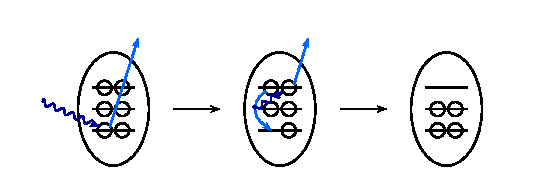
\includegraphics{pics/auger-pspic.eps}
 \caption{Schematic illustration of the Auger process. The initial vacancy is
          filled by an electron of an energetically higher orbital and the
          excess energy is transferred to another electron of the same atom,
          which is emitted.}
 \label{figure:auger_process}
\end{figure}

Special cases of the Auger process are the \ac{CK} and the \ac{SCK} decays.
In a \ac{CK} decay, the vacancy filling electron originates from a higher subshell
of the same shell characterized by the principal quantum number $n$. In a \ac{SCK}
decay the emitted electron also stems from the same shell. \cite{Coster35}

Since both the vacancy filling electron and the emitted electron originate
from the same atom as the initial vacancy, neither energy nor electrons need
to be transferred through space, this process is ultrafast with lifetimes
in the atto- to femtosecond region. \cite{}

In order to fulfill the energy criterion, the initial ionization energy has to
be high in order to exceed the final state energy. This is why
the process is rarely observed after
ionization from the inner-valence region and therefore, it is possibile to
observe other autoionization processes in the latter systems.

\section{\acl{ICD}}
The Interatomic/ Intermolecular Coulombic Decay (ICD) was predicted
theoretically 1997 by L. S. Cederbaum \cite{Cederbaum97}
and later verified experimentally by Marburger et al. \cite{Marburger03}.

Here the initial vacancy is filled by an electron of the same atom and simultaneously,
the atom interacts with the surroundings by
transferring the excess energy to another atom, which finally gets ionized. The
positive charges on the different atomic sites repell each other and therefore undergo
Coulomb explosion as shown in figure \ref{figure:icd_process}.

\begin{figure}[h]
 \centering
 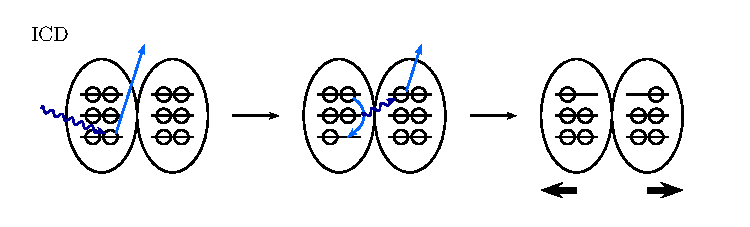
\includegraphics{pics/icd-pspic.eps}
 \caption{Schematic illustration of the \ac{ICD}. The initial vacancy is filled
          by an electron of the valence and the excess energy is transferred to
          an electron of a neighbouring atom, which consequently is emitted.
          The two positively charged units undergo Coulomb explosion.}
 \label{figure:icd_process}
\end{figure}

%For the following sections we introduce a new nomenclature. The combinations
%of all involved atoms and molecules is referred to as the (total) system, whereas
%each of them is named a unit. One or a conglomerat of these units, within
%the electron fills the vacancy is called a subsystem ($S_1$) as well as the units
%forming the 
%subsystem emitting the seconday electron $S_2$.

Due to the energy transfer via a virtual photon between to subsystems
the ICD has a lifetime of femto- to pico-seconds \cite{Zobeley98,Santra01_1,
Zobeley01,Santra01_3,Averbukh04,Averbukh05}.
The initial vacancy of observed ICD processes are normally in the inner-valence,
but are not limited to these cases. Nevertheless, one might rarely observe
an ICD after core ionization, because the Auger process would then be energetically
allowed and outrule the slower ICD.

An elaborate review including theoretical and experimental examples is to be
found in reference \cite{Hergenhahn11}.


\section{Electron Transfer Mediated Decay Processes}
In the \ac{ETMD} processes the vacancy is filled by an electron from another
atom or molecule. Depending on where
the excess energy is transferred to and
hence how many units are involved in the process, the processes are either called
ETMD2 or ETMD3 as shown in figure \ref{figure:etmd_processes}.

\begin{figure}[h]
 \centering
 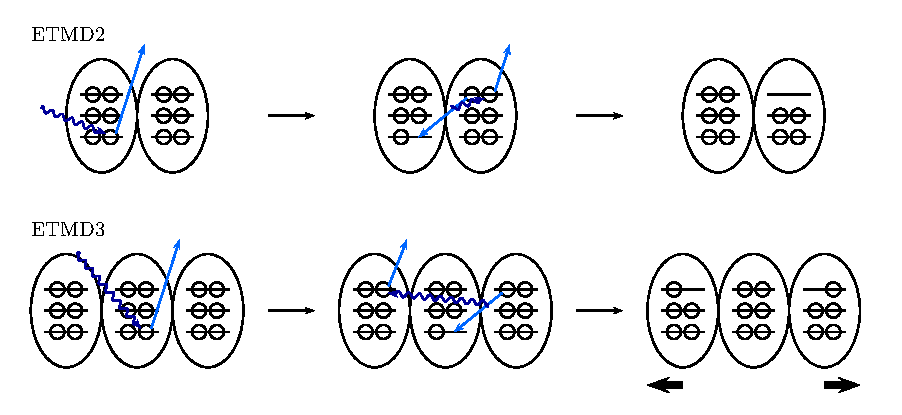
\includegraphics{pics/etmd-pspic.eps}
 \caption{Schematic representation of \ac{ETMD} processes. In the ETMD2 the initial
          vacancy is filled by an electron of a neighbouring atom and the excess
          energy is transferred to an electron of this second atom, which
          consequently gets ionized. The final state is charaterized by the initially
          ionized atom to be neutral and the neighbouring atom to be doubly ionized.
          In the \ac{ETMD}3, the initial vacancy is filled by an electron of a
          neighbouring unit and simultaneously the excess energy is transferred to
          an electron of a third unit, which gets ionized. The final state is
          characterized by the initially ioniued atom being neutralized and the
          two neighbouring atoms being singly ionized. Hence, the repell each other.}
 \label{figure:etmd_processes}
\end{figure}

In the ETMD2 \cite{Zobeley01} the excess energy is transferred an electron
from the vacancy filling unit while in the ETMD3 the excess energy is transferred
to a third unit \cite{Zobeley98}.

The decay rate of the process is mostly governed by the electron transfer rate, which
depends on the overlap between the electron clouds of the two units and hence
decreases exponentially with the internuclear/ intermolecular distance. Therefore,
the decay rate of the process is normally about two to three orders of magnitude slower
than a competing ICD process and can hence only be observed in cases where either
the ICD is energetically forbidden or, in case of the ETMD3, at interfaces
where the number of potential
triples of atoms is higher and therefore increases the probability for an ETMD3 process
\cite{Fasshauer13}.

The exchange ICD process' decay rate is also governed by the electron transfer
even though it is not evident from its name. As shown in
figure \ref{figure:exICD_process}, the innervalent vacancy is filled by an electron
from the second unit and the excess energy is then transferred back to the first,
initially ionized unit. The two positively charged units then undergo Coulomb
explosion.

\begin{figure}[h]
 \centering
 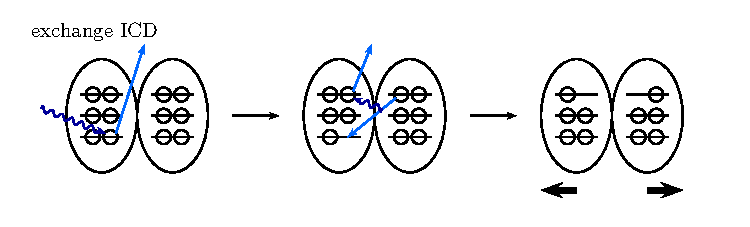
\includegraphics{pics/exicd-pspic.eps}
 \caption{Schematical illustration of the exchange \ac{ICD}. The initial
          vacancy is filled by an electron of the neighbouring unit and the
          excess energy is transferred to another electron of the initially ionized
          unit, which is emitted. The two positively charged units of the final
          state undergo Coulomb explosion.}
 \label{figure:exICD_process}
\end{figure}

Because the final state of the exchange ICD is the same as in the ICD the energy
criterion is the same as for the ICD and the final products are the same. Only
the decay rate is in the range of an ETMD process and hence the process is much
slower than an ICD process. Therefore it is not possible to experimentally
observe and identify this process independently. \cite{Zobeley01}


\section{Resonant ICD (RICD)}
Starting not from an ionized but from an electronically excited state, further
autoionization processes can be observed
as shown in figure \ref{figure:ricd_processes} panel a).
These electronic decay processes have been known for
the Auger process and been called resonant Auger effect. Analogously ICD like
processes can be initiated by an excitation, which also have been observed
experimentally. \cite{Barth05,Gokhberg06,Kopelke09}

\begin{figure}[h]
 \centering
 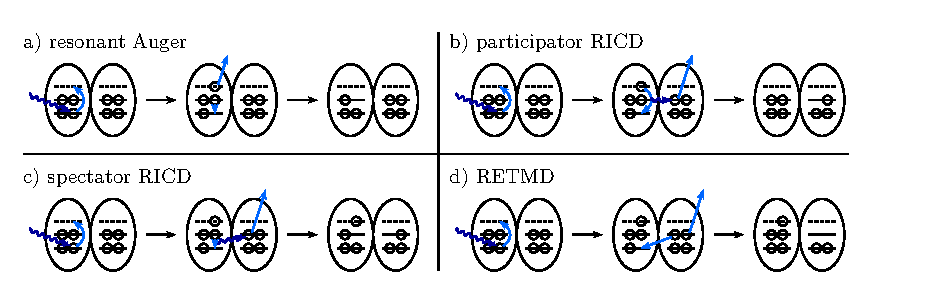
\includegraphics{pics/ricd-pspic.eps}
 \caption{Schematic illustration of resonant autoionization processes.
          For details see the main text.}
 \label{figure:ricd_processes}
\end{figure}

Depending on which role the excited
electron plays in the reaction, the process is either called participator \ac{RICD}
or spectator \ac{RICD}.
In a participator \ac{RICD} the excited electron fills the created vacancy itself.
Simultaneously the excess energy is transferred to a neighbouring unit, which
subsequently gets ioinzed (see figure \ref{figure:ricd_processes} panel b).
The final state is characterized
by the initially excited unit to be in its ground state and the neighbouring atom
being ionized.
In a spectator \ac{RICD} (see figure \ref{figure:ricd_processes} panel c)
the vacancy is filled by another, non-excited electron
of the same unit. The excess energy is simultaneously transferred to a neighbouring
unit, which is then ionized. Throughout the process the excited electron stays
in its virtual orbital.

Recently, the special case of a participator \ac{RICD} where the excited
electron stems not from the inner valence but from the outer valence
has been described and has been named \ac{ETI} \cite{Kopelke11}.

As in the case of an ionized initial state also the corresponding ETMD processes
called RETMD (see figure \ref{figure:ricd_processes} panel d) are possible.



